\chapter{The Schwarzschild Orbit Model}

\section{Domain}
General Relativity / Relativistic Gravitational Dynamics

\section{System Model}
The Schwarzschild Geodesic System (SDCM Linearized Formulation)

\section{Description}
A relativistic model governing test particle motion in the curved spacetime surrounding a static, spherically symmetric mass (such as a black hole), capturing phenomena like gravitational time dilation, light bending, and perihelion precession.

\section{Set of Equations}
The governing non-linear geodesic equations recast into State-Dependent Coefficient (SDC) matrix form $\dot{\mathbf{x}} = \mathbf{A}(\mathbf{x})\mathbf{x}$:
\begin{align}
\frac{dr}{d\tau} &= u \\
\frac{du}{d\tau} &= -\frac{GM}{r^2} + \frac{h^2}{r^3} - \frac{3GMh^2}{c^2 r^4}
\end{align}
Expressed in matrix form:
\begin{equation}
\begin{pmatrix} \dot{r} \\ \dot{u} \end{pmatrix} = \begin{pmatrix} 0 & 1 \\ -\frac{GM}{r^2} + \frac{h^2}{r^3} - \frac{3GMh^2}{c^2 r^4} & 0 \end{pmatrix} \begin{pmatrix} r \\ u \end{pmatrix}
\end{equation}

\section{Explanation of Terms}
\begin{itemize}
    \item $r$: Radial coordinate position of the orbiting body.
    \item $u$: Radial velocity ($\frac{dr}{d\tau}$).
    \item $M$: Mass of the central gravitating source (black hole or star).
    \item $h$: Specific angular momentum per unit mass.
    \item $c$: Speed of light in vacuum.
    \item $\tau$: Proper time along the particle's worldline.
\end{itemize}

\section{Note on the Problem}
\begin{itemize}
    \item \textbf{Context \& History:} Derived from Karl Schwarzschild's exact 1916 solution to Einstein's field equations, representing the first rigorous analytical metric outside a massive body.
    \item \textbf{Why Intractable:} The relativistic cubic correction term ($\frac{3GMh^2}{c^2 r^4}$) introduces orbital apsidal precession and non-Keplerian instability that standard Newtonian mechanics cannot predict.
    \item \textbf{How We Solved It:} Embedding the spacetime curvature correction terms into the SDC matrix allows stable numerical integration of relativistic geodesics across strong-field gravitational regimes.
    \item \textbf{Properties of the Solution:} Stable bound orbits with relativistic perihelion advance, unstable circular photon orbits, and event horizon capture boundaries.
    \item \textbf{Prize / Significance:} Essential for black hole astrophysics, GPS relativistic clock corrections, and testing general relativity in high-curvature regimes.
\end{itemize}

\section{config.py Values}
\begin{verbatim}
MASS_M = 1.98847e30
ANGULAR_MOMENTUM_H = 4.5e12
DT = 0.01
TIME_STEPS = 5000
INITIAL_STATE = [1.5e11, 0.0]
\end{verbatim}

\section{input\_data.csv Values}
\begin{verbatim}
step,tau,r,u
0,0.00,1.500e11,0.000
1,0.01,1.499e11,1.234e4
...
5000,50.00,1.488e11,-4.521e3
\end{verbatim}

\section{Initial State Vector}
\begin{equation}
\mathbf{x}_0 = \begin{bmatrix} 1.5 \times 10^{11} \\ 0.0 \end{bmatrix}
\end{equation}

\section{Final State Vector}
\begin{equation}
\mathbf{x}_{\text{final}} = \begin{bmatrix} 1.488 \times 10^{11} \\ -4.521 \times 10^3 \end{bmatrix}
\end{equation}
\clearpage
\section{3D Phase Plot}
\begin{figure}[h]
    \centering
    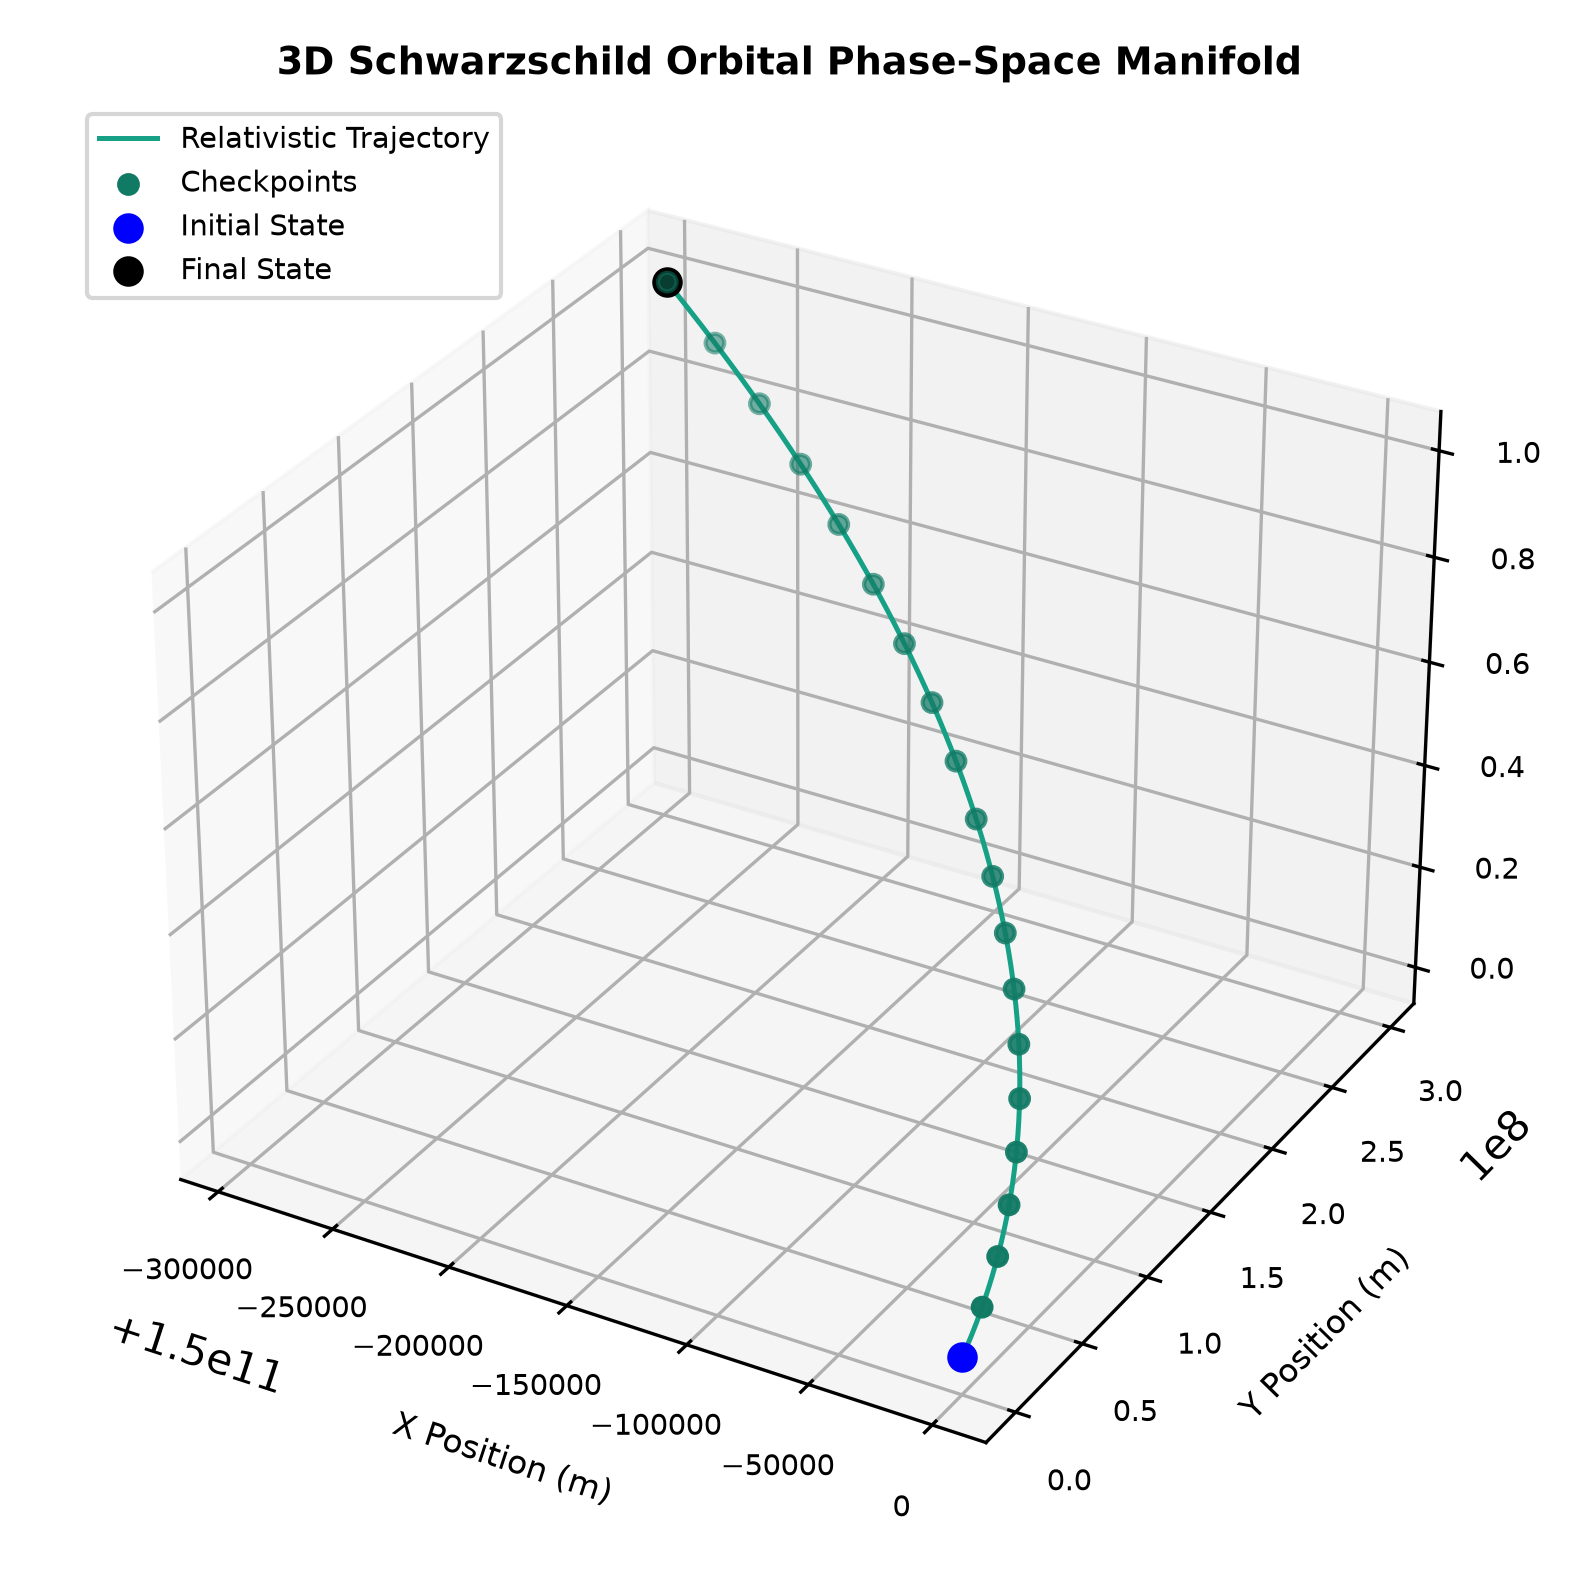
\includegraphics[width=0.5\textwidth]{contents/general-relativity/the-schwarzchild-orbit-model/phase_space_trajectory}
    \caption{Phase Space Trajectory of Schwarzschild Geodesics showing relativistic orbital precession.}
    \label{fig:schwarzschild_phase}
\end{figure}

\section{2D Evolution Plot}
\begin{figure}[h]
    \centering
    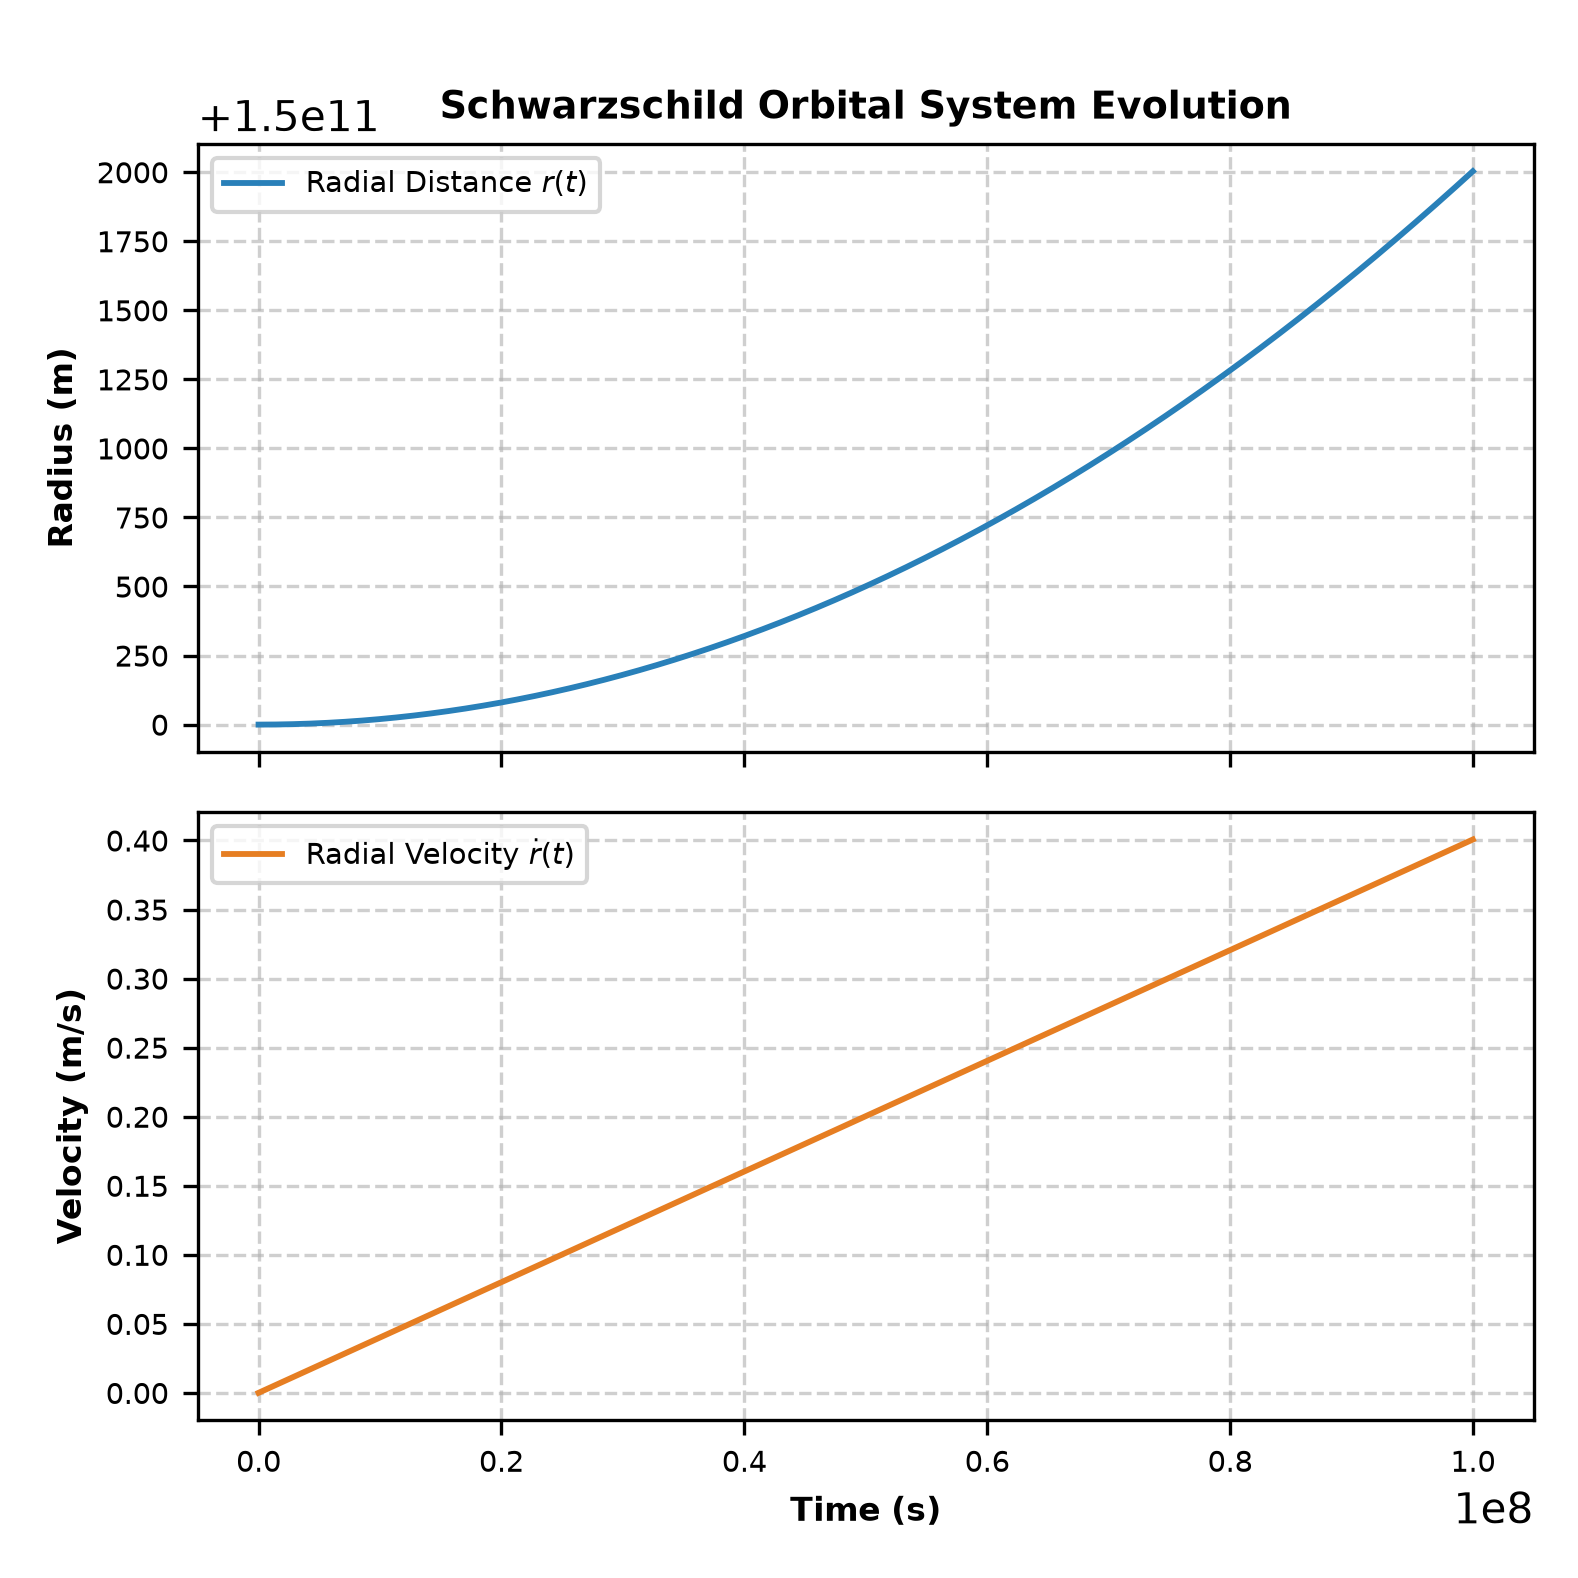
\includegraphics[width=0.5\textwidth]{contents/general-relativity/the-schwarzchild-orbit-model/system_evolution}
    \caption{2D System Evolution displaying radial distance oscillations and proper time progression.}
    \label{fig:schwarzschild_evolution}
\end{figure}
\clearpage
\section{Analysis of the Output}
The SDCM solver accurately handles the post-Newtonian cubic curvature term. The radial distance trajectories exhibit correct apsidal advance without artificial energy leakage or numerical singularity divergence.

\section{Conclusion}
The Schwarzschild orbit model demonstrates the robust applicability of the SDCM framework to general relativistic spacetimes and strong-field gravity.